\documentclass{article}
\usepackage[utf8]{inputenc}
\usepackage[papersize={8.5in,11in},margin=0.8in]{geometry}
\usepackage{xcolor}
\usepackage{color, colortbl}
\usepackage{graphicx}
\usepackage{tikz}
\usepackage{amssymb}
\usepackage{amsmath}
\usetikzlibrary{positioning}
\usetikzlibrary{graphs,graphs.standard}


\title{CS520 Written HW 1}
\author{John Caruthers}
\date\today

\begin{document}
\maketitle

\begin{itemize}
    \item[1] Given the DAG as below, answering the following question.
        \begin{center}
            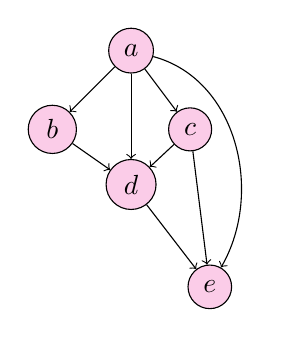
\begin{tikzpicture}
                [dot/.style = {draw,fill=magenta!20,circle}]
                
                \node[dot] (a) at (0, 0) {$a$};
                \node[dot] (b) at (-1,-1) {$b$};
                \node[dot] (c) at (0.75, -1) {$c$};
                \node[dot] (d) at (0, -1.7) {$d$};
                \node[dot] (e) at (1,-3) {$e$};
            
                \path[->] (a) edge (b);
                \path[->] (a) edge (c);
                \path[->] (a) edge (d);
                \path[->] (a) edge[out=345,in=60  ] (e);
                \path[->] (b) edge (d);
                \path[->] (c) edge (d);
                \path[->] (c) edge (e);
                \path[->] (d) edge (e);
            
            \end{tikzpicture}
        \end{center}
    \begin{itemize}
        \item[a)] Show the order of nodes visited with \textbf{breath first search} algorithm, starting at vertex \emph{a}.
        \item[b)] Show the order of nodes visited with \textbf{depth first search} algorithm, starting at vertex \emph{a}.
        \item[c)] Show the topological sort result.
    \end{itemize}
    \item[2.] Show the step-by-step result of growth of the minimum spanning tree when the following algorithms are performed on the graph below.
    \begin{center}
        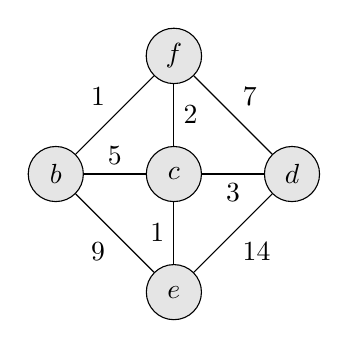
\begin{tikzpicture}
            [dot/.style = {minimum size = 0.7cm, draw, fill=gray!20, circle}]

            \node[dot] (f) at (0,0) {$f$};
            \node[dot] (c) at (0,-1.5) {$c$};
            \node[dot] (e) at (0,-3) {$e$};
            \node[dot] (b) at (-1.5,-1.5) {$b$};
            \node[dot] (d) at (1.5,-1.5) {$d$};

            \draw[-] (c) to node[right] {2} (f);
            \draw[-] (c) to node[below] {3} (d);
            \draw[-] (c) to node[left] {1} (e);
            \draw[-] (c) to node[above] {5} (b);
            \draw[-] (b) to node[above left] {1} (f);
            \draw[-] (b) to node[below left] {9} (e);
            \draw[-] (d) to node[above right] {7} (f);
            \draw[-] (d) to node[below right] {14} (e);
            
        \end{tikzpicture}
    \end{center}
    \begin{itemize}
        \item[a)] Kruskal's algorithm.
        \item[b)] Prim's algorithm (indicate starting node).
    \end{itemize}
\end{itemize}

\end{document}
